\section{O que as médias escondem}
\begin{figure}[H]
\centering
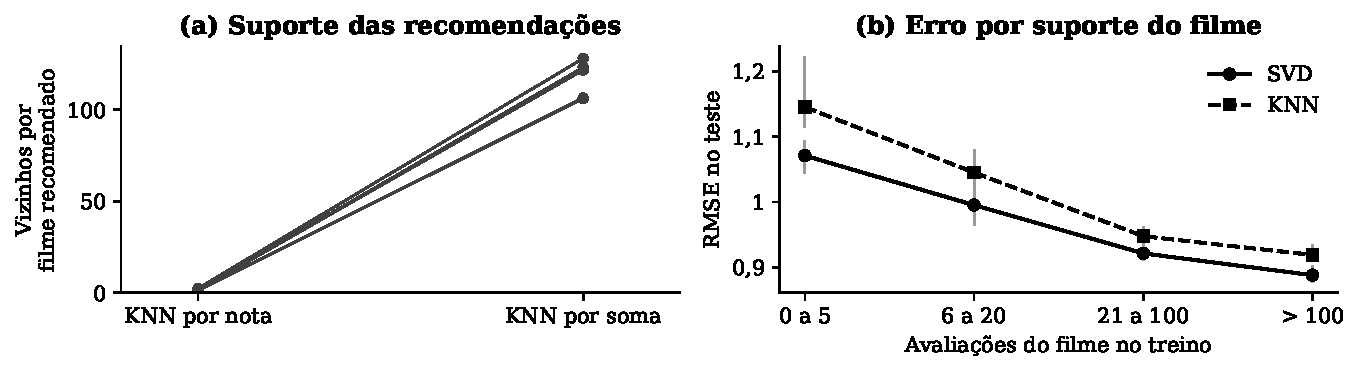
\includegraphics[width=\textwidth]{figuras/ativ_diagnostico.pdf}
\caption{(a) Vizinhos que avaliaram cada recomendado: média por lista, uma
linha por partição. (b) RMSE por suporte no treino: pontos são médias entre
partições; segmentos, mínimos e máximos.}
\label{fig:diagnostico}
\end{figure}

O KNN por nota apoia cada recomendação em \vizNota\ vizinhos, em média, contra
\vizSoma\ na soma. Os filmes escolhidos têm, respectivamente, \avalNota\ e
\avalSoma\ avaliações no treino. A normalização permite notas altas com poucos
vizinhos; a soma retém o volume de evidência. O contraste sugere fragilidade
com pouco suporte, mas não separa esse efeito da preferência por filmes populares.

O SVD tem menor RMSE em todas as faixas de suporte e nas cinco partições
(Figura~\ref{fig:diagnostico}b). Porém, apenas \nPoucoSuporte\ notas de teste envolvem
filmes com até cinco avaliações no treino, contra \nMuitoSuporte\ com mais de 100:
o erro agregado representa sobretudo filmes com mais histórico.

\begin{figure}[H]
\centering
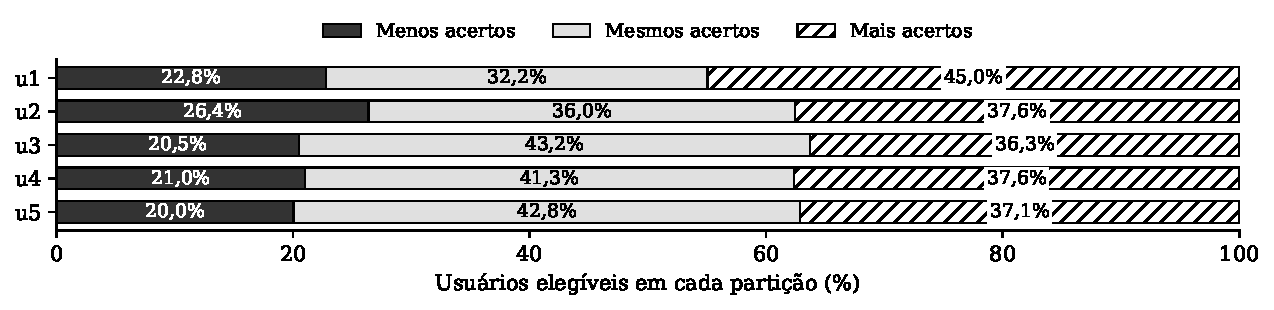
\includegraphics[width=0.92\textwidth]{figuras/ativ_usuarios.pdf}
\caption{KNN por soma versus popularidade: usuários com menos, iguais ou mais
acertos por lista em cada teste externo.}
\label{fig:usuarios}
\end{figure}

\textbf{O ganho médio não beneficia todos.} Em média entre partições,
\vence\% ganham acertos, \empata\% empatam e \perde\% perdem. Os mesmos
usuários podem reaparecer em diferentes partições.
